\documentclass[../main.tex]{subfiles}
\graphicspath{{\subfix{../figures/}}}
% \addbibresource{../bibliografia/bibliografia.bib}
% \addbibresource{../bibliografia/TFG.bib}
    
% \usepackage[showframe]{geometry}
% \usepackage{sidecap}
% \sidecaptionvpos{figure}{t}

\begin{document}

\chapter{Design of the Solution} \label{chap:methodology}
    % \section{Technical Approach} \label{technical_approach}
        
    % \section{Aspects considered} \label{aspects_considered}

    This work is driven by the problem of designing platforms primarily used to perform Machine-Learning inference (only obtaining the output predictions from a model) while ensuring that the obtained outputs are as reliable and robust as possible when encountering new data. This is important in scenarios where a model is deployed in high-stake environments 
    where their output causes significant downstream impact, and inaccurate predictions may be costly to the relevant stakeholders.
    
    We consider that these types of platforms have the following characteristics:

    \begin{itemize}
        \item The (already trained) models are uploaded to the platform primarily to obtain predictions from new data. We refer to the bag of models available to the platform as the \textit{model repository}.
        \item  The data used to train and evaluate the models is available. This means the platform can have prior knowledge about the data distribution the models were trained on.
        % \item The training environment is detached from the inference environment. That is, we go with the assumption that the models are trained in a different environment than the one where they are deployed.
        \item The platform has enough hardware resources available to perform inference with the models that it has available. 
        % Furthermore, the inference is considered to be computationally cheap compared to the training phase.
        \item The platform constantly receives new data for inference, which is assumed to be independent of the data used to train the models.
        \item Labeling capabilities are limited. That is, annotating new data is costly and unfeasible in large amounts.  This is common in real-world applications, notably in the healthcare sector, where the labeling task is performed by professional workers, making it a costly and time-consuming task
        \cite{yakimovich_labels_2021,chen_study_2015, figueroa_predicting_2012}.
    \end{itemize}

    Furthermore, for the purpose of this work, we consider that the inference environment is deployed alongside an \textit{experimental} environment. This environment is assumed to be detached from the training environment and is set up to continuously evaluate the models' robustness on new data, evaluate its performance after retraining using the aforementioned techniques, and compare the results with the deployed model. If the experimental model outperforms the deployed model, the latter is updated with the new model. This process is repeated for the entire lifetime of the application.


    The role of the human annotator in designing machine-learning models is also an important aspect of this work...

    \begin{figure}[t]
        \centering
        \caption{Diagram of the Proposed System}
        \hspace*{-0.3cm}
        \resizebox*{1.15\columnwidth}{!}{
            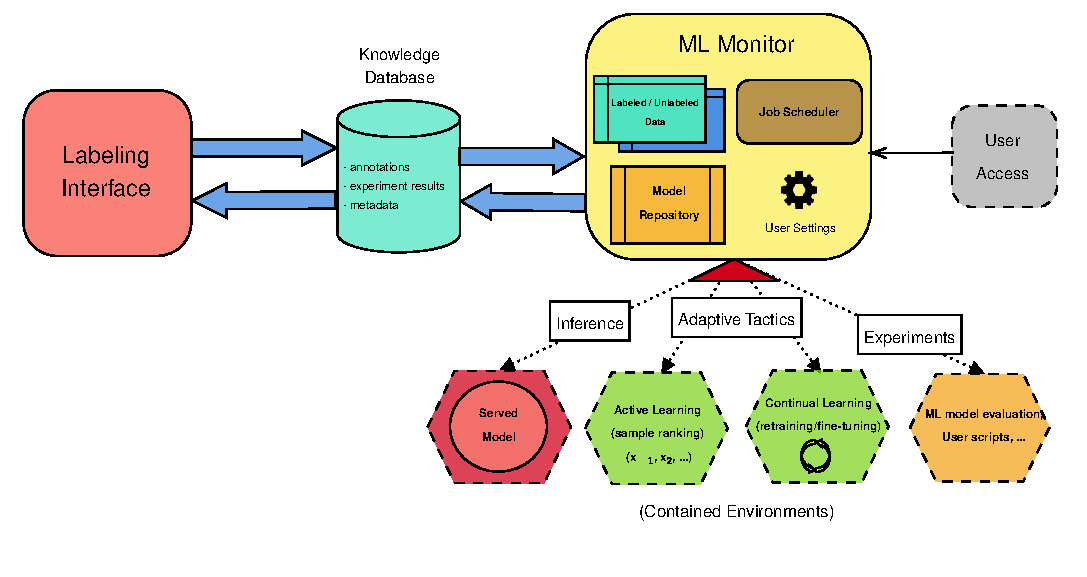
\includegraphics{ml_system_proposal.pdf}
        }
        \label{fig:system_proposal_diagram}
    \end{figure}

        
  
% \printbibliography
\end{document}